\documentclass[aspectratio=169,10pt,xcolor=pdflatex,dvipsnames,table]{beamer}
\usepackage{newcent}
\usepackage[utf8]{inputenc}
\usepackage[shorthands=off,czech]{babel}
\usepackage{hyperref}
\usepackage{amsthm}
\usepackage{amssymb}
\usepackage{amsmath}
\usepackage{array}
\usepackage{stmaryrd}
\usepackage{graphicx}
\usepackage{tabularx}
\usepackage{listings}
\usepackage{fancyvrb}
\usepackage{minted}
%\usepackage{packages/beamerthemeFIT}

\makeatletter
  \def\beamer@calltheme#1#2#3{%
    \def\beamer@themelist{#2}
    \@for\beamer@themename:=\beamer@themelist\do
    {\usepackage[{#1}]{\beamer@themelocation/#3\beamer@themename}}}

  \def\usefolder#1{
    \def\beamer@themelocation{#1}
  }
  \def\beamer@themelocation{}

\usefolder{packages}
\usetheme{FIT}

\title[OpenGL]{PGR - GPU, Rendering pipeline, OpenGL}

\author[]{Tomáš Milet}

\institute[]{Brno University of Technology, Faculty of Information Technology\\
Bo\v{z}et\v{e}chova 1/2. 612 66 Brno - Kr\'alovo Pole\\
imilet@fit.vutbr.cz}

\date{\today}

\begin{document}

\frame[plain]{\titlepage}

\definecolor{bg}{rgb}{0.95,0.95,0.95}

\bluepage{Overview of GPU architecture / Přehled architektury GPU}

\begin{frame}
\frametitle{GPU over the years / GPU architektura v průběhu let}
  \scriptsize
	\begin{itemize}
	\item At first, everything was fixed in HW / just 2D acceleration.
	\item 3D acceleration next, specialized HW.
	\item Next, partially programable pipeline.
  \item Now, large number of cores for general computation, (2D emulated).
	\end{itemize}
	\begin{itemize}
	\item Nejprve pouze 2D akcelerace
	\item Poté 3D akcelerace, specializovaný HW
	\item Dál částečně programovatelná pipeline
	\item Nyní velké množství výpočetních jednotek pro obecné výpočty (2D akcelerace emulovaná pomocí 3D)
	\end{itemize}
	\begin{figure}[h]
	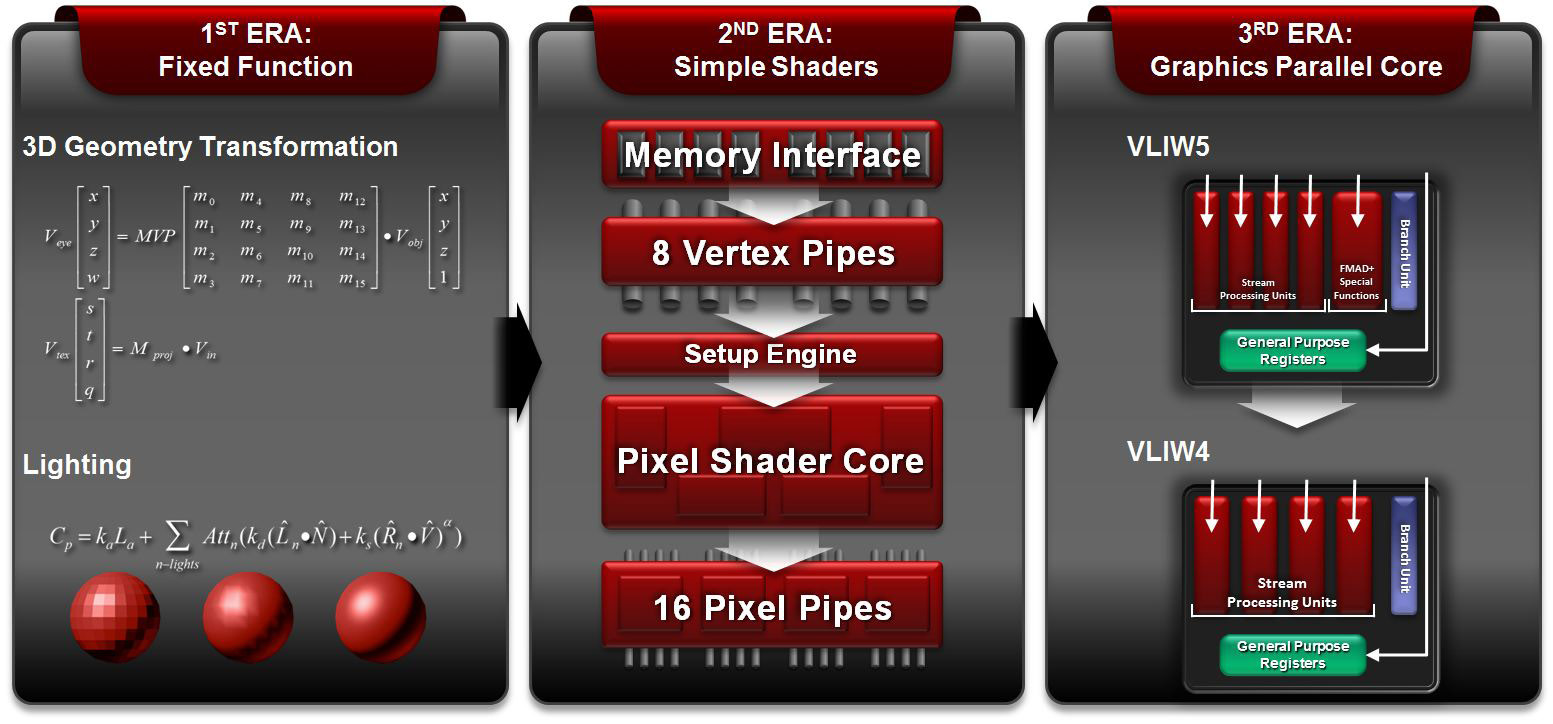
\includegraphics[width=10cm,keepaspectratio]{pics/gpu/gpu_amdevoluce}
	\end{figure}
\end{frame}

\begin{frame}
\frametitle{GPU vs CPU}
  \scriptsize

	\begin{itemize}
	\item CPU - small number of very fast computing units.
	\item Large caches, large control, out-of-order instruction execution, ...
	\item GPU - large number of not that fast computing units, simpler units.
	\item Smaller caches, small control, more transistors allocated for computation, ...
  \item GPU - data parallel, semi tast parallel
  \item CPU - tast parallel, semi data parallel
	\end{itemize}

	\begin{itemize}
	\item CPU - málo, velmi výkonných výpočetních jednotek
	\item Velká keš, velké řízení, vykonávání instrukcí mimo pořadí, ...
	\item GPU - velké množství méně výkonných, jednodušších výpočetních jednotek
	\item Malé keše, malé řízení, víc tranzistorů pro výpočty, ...
  \item GPU - data parallel, náznak task parallel
  \item CPU - tast parallel
	\end{itemize}
	\begin{figure}[h]
	
\includegraphics[width=10cm,keepaspectratio]{pics/gpu/gpu_gpuvscpu.pdf}
	\end{figure}
\end{frame}

\begin{frame}
\frametitle{GPU vs CPU}
	\begin{figure}[h]
	
\includegraphics[width=10cm,keepaspectratio]{pics/gpu/gpu_common}
	\end{figure}
  \scriptsize

	\begin{itemize}
	\item GPU is composed from multi-processors and device memory.
  \item Nvidia - streaming multi processor (SM).
  \item AMD   - compute unit (CU).
  \item Multi-processor is composed of SIMD units and various kings of memory.
  \item Computation executed on one multi-processor is independed from computation on other multi-processors.
  \item SIMD cores are commony reffered as shader unit (AMD Radeon HD7970M 20xCU, 64 shader unit per CU, = 1280 shader unit).
	\end{itemize}

	\begin{itemize}
	\item Grafická karta je složena z několika multiprocesorů a grafické paměti.
  \item Nvidia - streaming multi processor (SM).
  \item AMD   - compute unit (CU).
  \item Tento multiprocessor je dále složen z velkého množství jader a různých druhů pamětí.
  \item Akce, která beží na jednom multiprocesoru je nezávislá na akci, která běží na jiném multiprocesoru.
  \item Jádra bývají označována jako shader unit (AMD Radeon HD7970M 20xCU, 64 shader unit na CU, = 1280 shader unit).
	\end{itemize}
\end{frame}

\begin{frame}
\frametitle{NVIDIA - GTX 1080}
	\begin{figure}[h]
	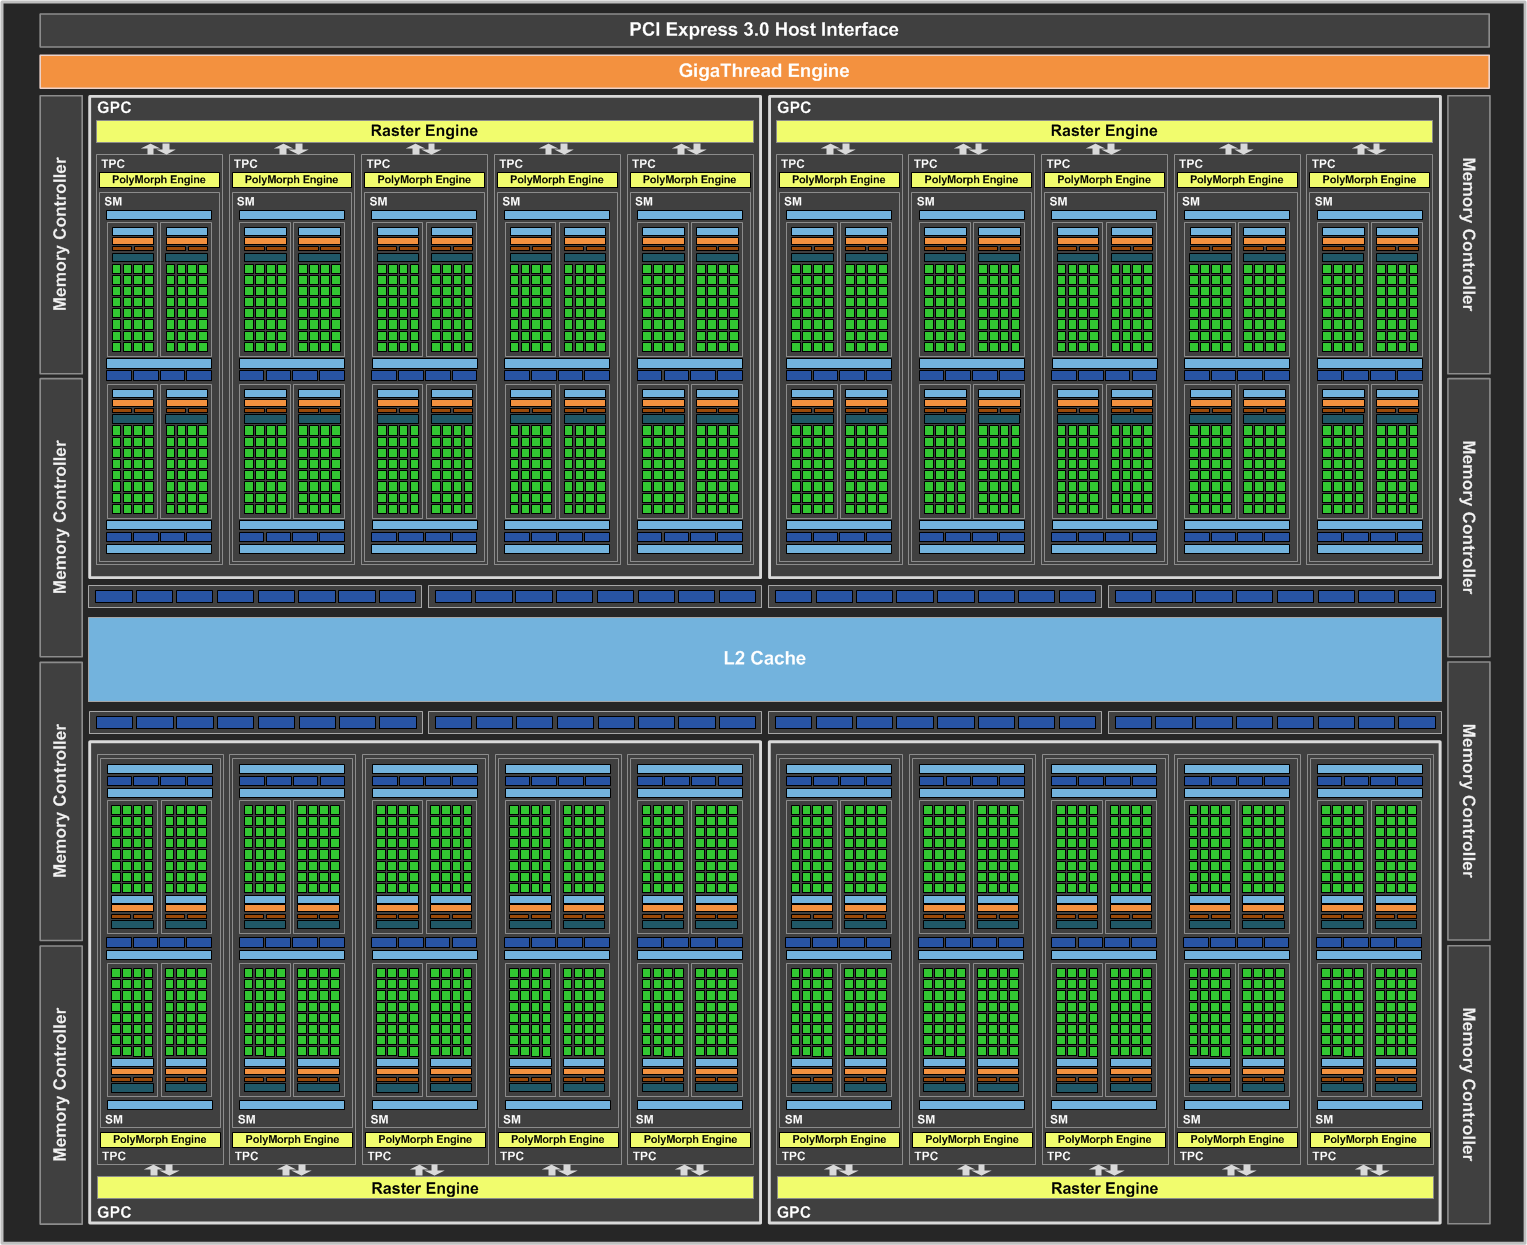
\includegraphics[width=8.5cm,keepaspectratio]{pics/gpu/1080}
	\end{figure}
\end{frame}

\begin{frame}
\frametitle{AMD FuryX/fiji}
	\begin{figure}[h]
	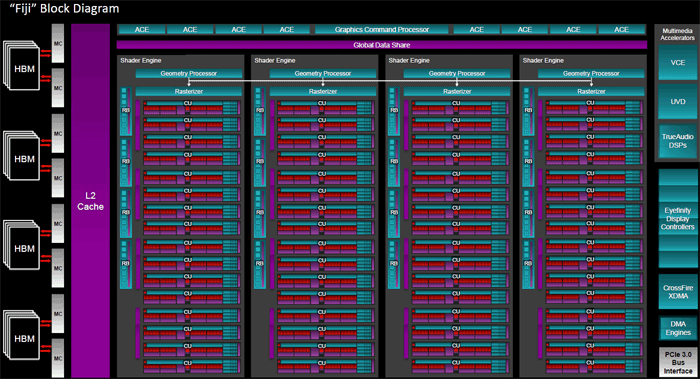
\includegraphics[width=11cm,keepaspectratio]{pics/gpu/furyx}
	\end{figure}
\end{frame}

\begin{frame}
\frametitle{NVIDIA - Fermi SMX}
	\begin{figure}[h]
	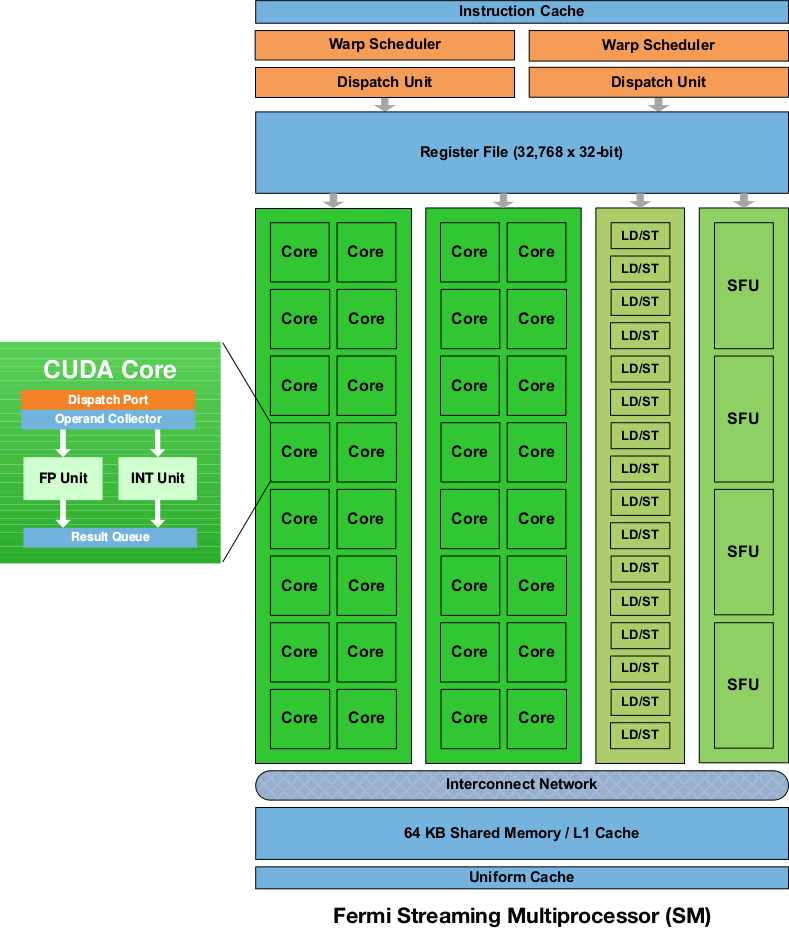
\includegraphics[width=7cm,keepaspectratio]{pics/gpu/fermi}
	\end{figure}
\end{frame}

\begin{frame}
\frametitle{NVIDIA - 1080 SMX}
	\begin{figure}[h]
	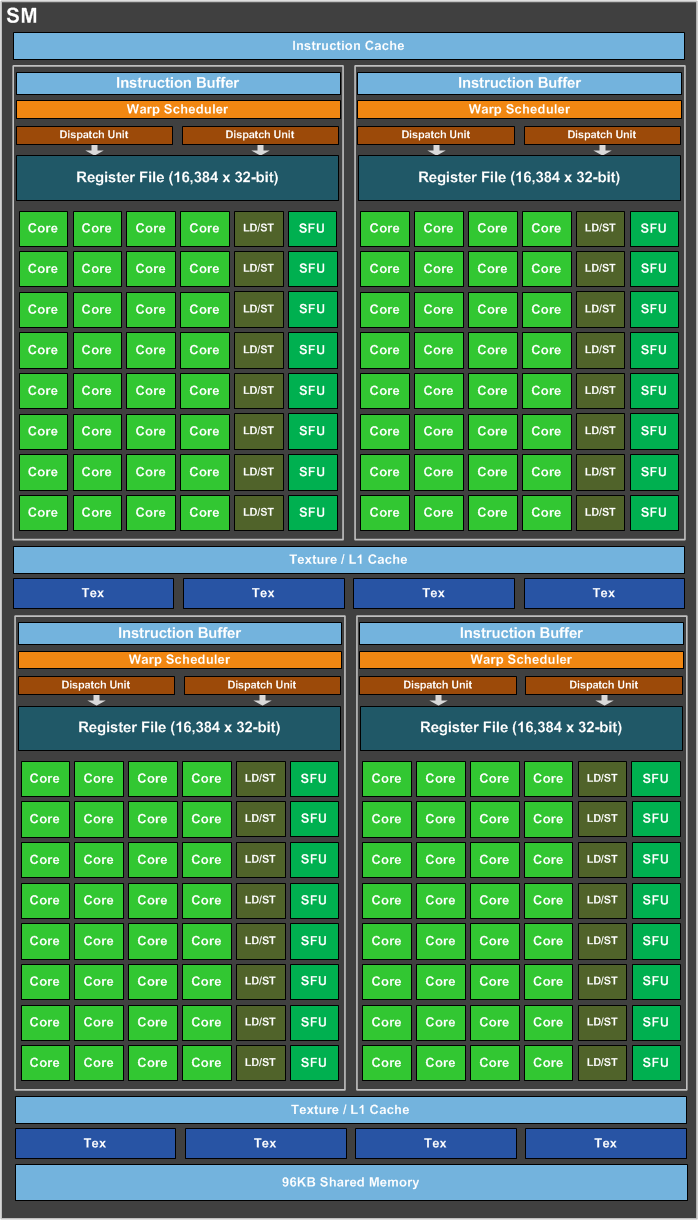
\includegraphics[width=4.5cm,keepaspectratio]{pics/gpu/1080SMX}
	\end{figure}
\end{frame}

\begin{frame}
\frametitle{AMD - GCN}
	\begin{figure}[h]
	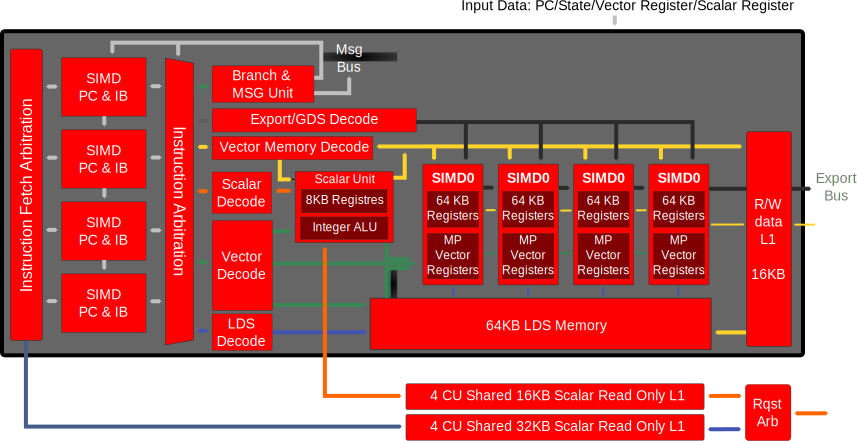
\includegraphics[width=11cm,keepaspectratio]{pics/gpu/gcn}
	\end{figure}
\end{frame}

\begin{frame}
\frametitle{Non programable parts of GPU / Hardwarové části}
  \scriptsize
	\begin{itemize}
	\item Today's GPUs are highly programable.
  \item Few parts remain fixed for configurable.
  \item Rasterization - converting vector primitives to fragments.
  \item Tessellation - splitting polygons into many sub-polygons.
  \item Texture units - filtering, wraping, compression, ...
  \item Per-fragment-operation, depth buffer, stencil buffer, ...
  \item Ray-tracing, ...
  \item And more
  \item Some parts are inaccessible from some APIs (CUDA cannot use rasterization).
	\end{itemize}
	\begin{itemize}
	\item Dnešní GPU jsou značně programovatelné
  \item Některé části stále zůstávají hardwarově zadrátované
  \item Rasterizace - převod trojúhelníků na fragmenty
  \item Tessellace - rozřezání polygonů na mnoho podpolygonů
  \item Texturovací jednoty - filtrování, opakování na okrajích, ...
  \item Depth buffer, Stencil buffer, ...
  \item A další
  \item Ke většině lze přistoupit pouze z některých API (OpenGL, Vulkan, DirectX)
	\end{itemize}
\end{frame}

\begin{frame}
  \frametitle{Memory Hierarchy / Paměťová hierarchie}
  \begin{columns}[T]
    \begin{column}{.48\textwidth}
      \begin{figure}[h]
        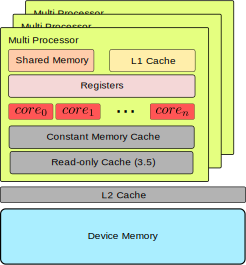
\includegraphics[width=5cm,keepaspectratio]{pics/gpu/memory_hierarchy}
      \end{figure}
    \end{column}
    \begin{column}{.48\textwidth}
      \scriptsize
      \begin{itemize}
        \item Different memory types with different size and speed.
        \item General rule: closer to core, faster, smaller memory.
        \item Registers are fastest (Ada contains 256KB of registers per SM).
        \item Shared/Local memory is used for thread communication.
        \item Device memory/global memory is cached using L2 cache. Large, big latency (100s of clocs).
      \end{itemize}

      \begin{itemize}
        \item Spousta různých pamětí s různou velikostí a rychlostí.
        \item Obecně platí, čím blíže k jádru, tím rychlejší a tím menší.
        \item Registry jsou nejrychlejší (na Ada je 256KB registrů na SM).
        \item Sdílená paměť slouží pro komunikaci mezi vlákny.
        \item Device memory (global memory) je velká (16GB i více), ale pomalá paměť.
      \end{itemize}
    \end{column}
  \end{columns}
\end{frame}

\begin{frame}
  \frametitle{Thread Hierarchy / Vláknová hierarchie}
  \scriptsize
  \begin{itemize}
    \item Thread is kernel instantion with unique index.
    \item Kernel/Shader is program composed of instruction.
    \item User launches 1000s of threads - Dispatch.
    \item Dispatch is divided into work-groups. Whole work-group runs on one SM.
    \item WG are further divided into Warps/Wavefronts (32/64 threads sub-groups).
    \item Warps/Wavefronts are executed on SIMD unit. (One warp per one SIMD).
    \item Threads in WG can be synchronized and can use shader memory.
    \item WG are 1D, 2D, 3D (dictates thread ordering and indices).
    \item Terminology differs (OpenCL, Cuda, Compute Shader, ...).
  \end{itemize}
  \begin{itemize}
    \item Na GPU pouštíme instance kernelů - vlákna.
    \item Kernel je program složený z instrukcí (podobně jako shader) a běží ve vláknu.
    \item Instrukce v kernelu jsou spouštěny v mnoha instancích na jádrech SM.
    \item Vlákna (thread, invocation, work-item) jsou seskupovány do pracovních skupin (work-group).
    \item Vlákna v pracovních skupinách můžou být na sobě závislá.
    \item Skupiny můžou být 1D, 2D, 3D (určuje pořadí vláken a jejich index).
    \item Mnoho work-group tvoří dispatch (taky může být 1D, 2D, 3D).
    \item Terminologie se liší (OpenCL, Cuda, Compute Shader, ...).
  \end{itemize}
\end{frame}

\begin{frame}
  \frametitle{Compute shader}
  \begin{picture}(320,250)
		\put(-28,50){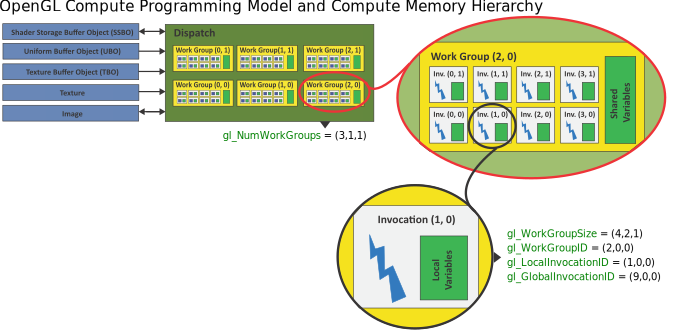
\includegraphics[height=6.4cm]{pics/gpu/threadHierarchy}}
	\end{picture}
\end{frame}

\begin{frame}
  \frametitle{Thread Hierarchy / Vláknová hierarchie}
  \begin{figure}[h]
	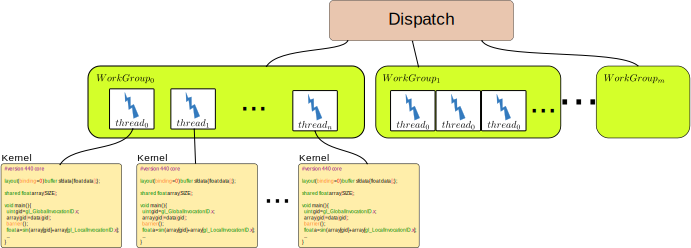
\includegraphics[width=11cm,keepaspectratio]{pics/gpu/thread_hierarchy}
	\end{figure}
  \scriptsize

  \begin{itemize}
    \item Threads are grouped to work-groups.
    \item Work-group can be 1D, 2D, 3D.
    \item WG are grouped into dispatch.
    \item Dsipatch can also be 1D, 2D, 3D.
    \item One SM can lauch multiple work-groups, if there is enough resourses (registers, shader memory).
  \end{itemize}

  \begin{itemize}
    \item Vlákna jsou seskupena do skupin work-group.
    \item Work-group může být 1D, 2D, 3D.
    \item Work-groupy jsou seskupeny do dispatch.
    \item Dispatch může být také 1D, 2D, 3D.
    \item Na jeden SM se může pustit vícero Work-group, pokud na to vystačí zdroje (registry, sdílená paměť)!
  \end{itemize}
\end{frame}


\bluepage{Reprezentace modelu}

\begin{frame}
\frametitle{Reprezentace scény}
	\begin{itemize}
		\item{Povrchová reprezentace - vektorová data.}
	\end{itemize}
	\begin{figure}[h]
		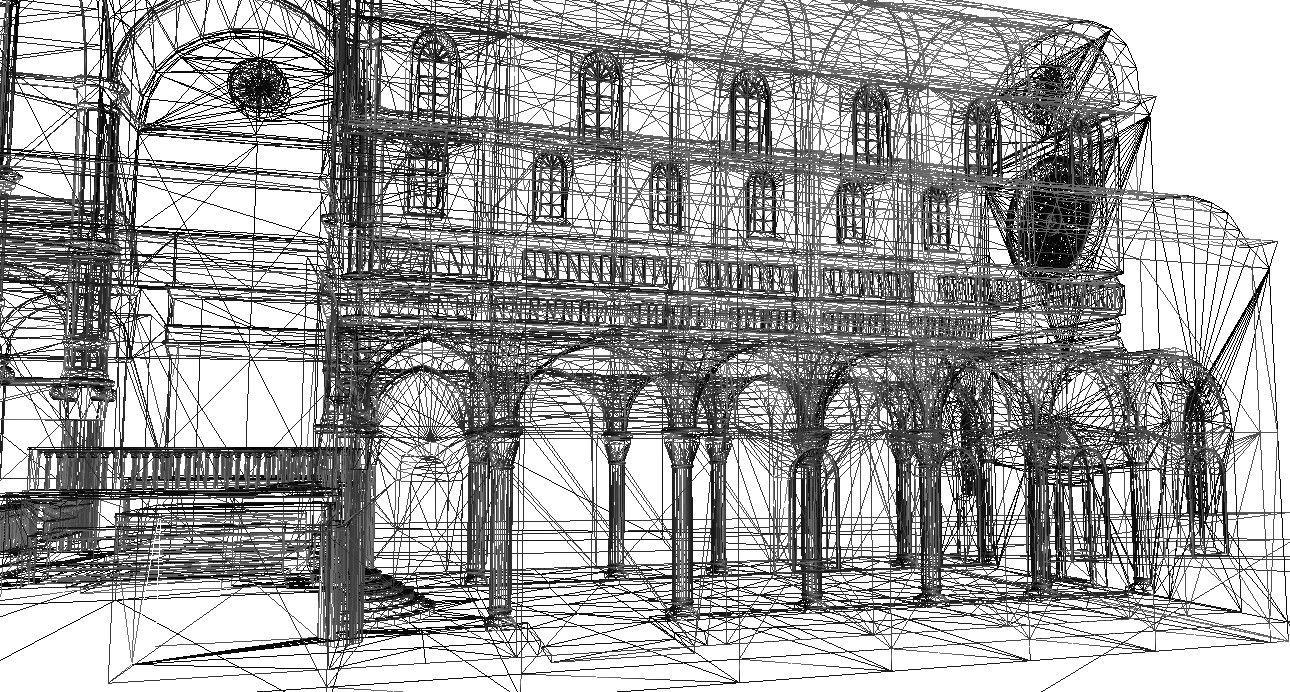
\includegraphics[width=10cm,keepaspectratio]{pics/model/wireframe.jpg}
	\end{figure}
\end{frame}

\begin{frame}
\frametitle{Reprezentace scény}
	\begin{itemize}
		\item{OpenGL pracuje s vrcholy - Vertexy}
		\item{Jeden Vertex může obsahovat několik různých atributů (pozice, barva, čas, hmotnost, texturovací koordináty,...)}
		\item{Několik Vertexů tvoří jedno primitivum - bod, úsečka, trojúhelník,...}
	\end{itemize}
	\begin{figure}[h]
		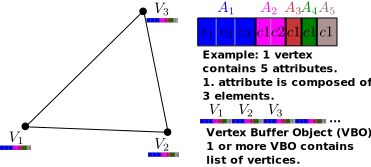
\includegraphics[width=10cm,keepaspectratio]{pics/model/primitive.pdf}
	\end{figure}
\end{frame}



\bluepage{Rendering Pipeline / Zobrazovací řetězec}

\begin{frame}
\frametitle{GPU / Rendering Pipeline / Zobrazovací řetězec}
  \scriptsize
	\begin{itemize}
		\item GPU is divided into memory and rendering pipeline.
	\end{itemize}
	\begin{itemize}
		\item GPU je rozděleno na paměť a vykreslovací řetěžec.
	\end{itemize}
	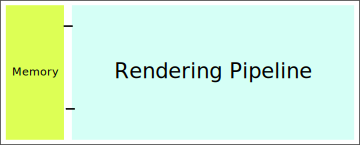
\includegraphics[width=12.5cm,keepaspectratio]{pics/pipeline/RenderingPipelineMemoryPipeline}
\end{frame}

\begin{frame}
\frametitle{Rendering Pipeline / Zobrazovací řetězec}
  \scriptsize
	\begin{itemize}
		\item Rendering Pipeline is divided into 2 parts: vector and raster.
    \item Splitting element is rasterization.
	\end{itemize}
	\begin{itemize}
		\item Zobrazovací řetěžec je rozdělen na 2 části - vektorovou a rastrovou.
    \item Dělícím prvkem je rasterizace.
	\end{itemize}
	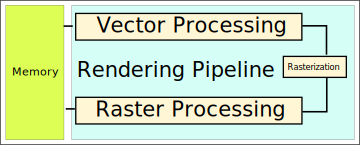
\includegraphics[width=12.5cm,keepaspectratio]{pics/pipeline/RenderingPipelineVectorRaster}
\end{frame}

\begin{frame}
\frametitle{Vector Part / Vektorová část}
  \scriptsize
	\begin{itemize}
		\item The main goal of vector part is to transform geometry.
    \item It processes vertices, primitives, it performs transformations, clipping, cullling, tessellation, projection,...
	\end{itemize}

	\begin{itemize}
		\item Hlavním úkolem vektorové části je transformace geometrie.
    \item Počítá vertex, primitiva, provádí transformace, ořez, teselaci, projekci, ...
	\end{itemize}

	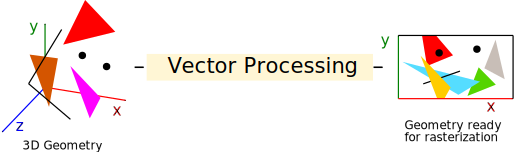
\includegraphics[width=12.5cm,keepaspectratio]{pics/pipeline/pipeline_vector_overview}
\end{frame}

\begin{frame}
\frametitle{Rasterization / Rasterizace}
  \scriptsize
	\begin{itemize}
    \item The goal of rasterization is to convert vector graphics elements (triangles, lines, points) to fragments.
	\end{itemize}

	\begin{itemize}
    \item Cílem rasterizace je převod vektorových grafických elementů (trojúhelníky, čáry, body) na fragmenty.
  \end{itemize}
	
\includegraphics[width=12.5cm,keepaspectratio]{pics/pipeline/rasterization_overview}
\end{frame}

\begin{frame}
\frametitle{Raster Part / Rastrová část}
  \scriptsize
	\begin{itemize}
		\item The main goal of raster part is to process fragments.
    \item It colors fragment, performs per fragment operations, depth test, stencil test, blending, ...
	\end{itemize}

	\begin{itemize}
		\item Hlavním úkolem rastrové části je výpočet fragmentů.
    \item Obarvuje fragment, provádí per fragment operace, hloubkový test, stencil test, blending, ...
	\end{itemize}
  
\includegraphics[width=12.5cm,keepaspectratio]{pics/pipeline/pfo_overview}
\end{frame}


\begin{frame}
\frametitle{Vector Part / Vektorová část}
  \scriptsize
	\begin{itemize}
		\item Vector Part is composed of many blocks.
    \item Some of the blocks are programable, some can be skipped.
	\end{itemize}
	\begin{itemize}
		\item Vektorová část řetězce je složena z mnoha bloků.
    \item Některé bloky jsou programovatelné a některé vynechatelné.
	\end{itemize}
	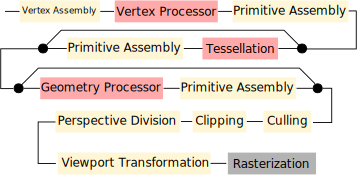
\includegraphics[width=12.5cm,keepaspectratio]{pics/pipeline/RenderingPipelineVector}
\end{frame}

\begin{frame}
\frametitle{Simplified vector part / Zlednodušená Vektorová část}
  \scriptsize
	\begin{itemize}
		\item If we remove optional blocks, the pipeline looks like this.
	\end{itemize}
	\begin{itemize}
		\item Pokud vynecháme volitelné bloky, zůstane zjednodušená vektorová část řetězce.
	\end{itemize}
	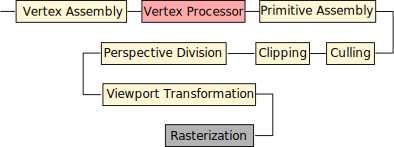
\includegraphics[width=12.5cm,keepaspectratio]{pics/pipeline/simplified_pipeline}
\end{frame}

\begin{frame}
\frametitle{Vertex Assembly, vertex processor, primitive assembly}
  \scriptsize
	\begin{itemize}
		\item Vertex Assembly creates vertices.
    \item Vertex processor transforms vertices.
    \item Primitive assembly creates base primitives from transformed vertices.
  \end{itemize}
	\begin{itemize}
		\item Vertex Assembly sestavuje vrcholy
    \item Vertex processor transformuje vrcholy
    \item Primitive assembly sestavuje základní primitiva.
	\end{itemize}
	
\includegraphics[width=12.5cm,keepaspectratio]{pics/pipeline/OpenGL460PipelineVertexShader}
\end{frame}

\begin{frame}
\frametitle{Vertex, Vertex Assembly}
  \scriptsize
	\begin{itemize}
		\item Vertex is a structure of vertex attributes.
    \item Vertex Assembly unit reads data from memory and forms vertices.
	\end{itemize}

	\begin{itemize}
		\item Vertex je struktura vertex atributů
    \item Vertex Assembly jednotka se stará o sestavování vrcholů z bufferů.
	\end{itemize}
	\begin{picture}(120,150)
		\put(0,0){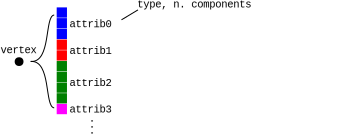
\includegraphics[width=12.5cm,keepaspectratio]{pics/pipeline/vertex}}
	\end{picture}
	\begin{picture}(60,40)
		\put(50,0){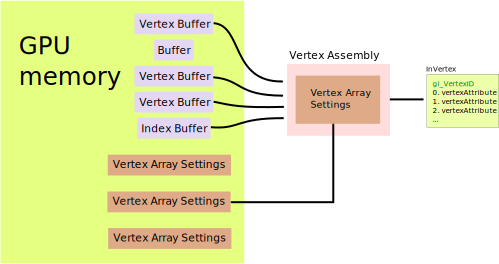
\includegraphics[width=8cm,keepaspectratio]{pics/pipeline/vertexAssembly}}
	\end{picture}
\end{frame}

\begin{frame}
\frametitle{Vertex Assembly / indexing}
  \scriptsize
	\begin{itemize}
		\item Vertex Assembly can utilize indexing
    \item Vertex Cache - already processed vertices do not have to be processed again
	\end{itemize}
	\begin{itemize}
		\item Vertex Assembly může využít indexování
    \item Vertex Cache - jednou propočítané vrcholy není třeba počítat znovu
	\end{itemize}
	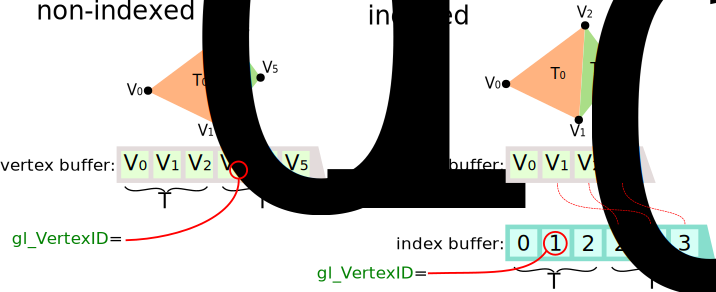
\includegraphics[width=12.5cm,keepaspectratio]{pics/pipeline/drawElements}
\end{frame}

\begin{frame}
\frametitle{Vertex Processor}
  \scriptsize
	\begin{itemize}
		\item Vertex Processor executes vertex shader.
    \item Vertex Shader is user program.
    \item The goal is to transform input vertex structure to output vertex structure.
	\end{itemize}

	\begin{itemize}
		\item Ve Vertex Processoru běží vertex shader.
    \item Vertex Shader je uživatelem specifikovaný program.
    \item Cílem je transformovat vstupní vrchol na výstupní vrchol.
	\end{itemize}
	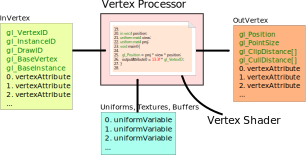
\includegraphics[width=10.5cm,keepaspectratio]{pics/pipeline/vertexShader}
\end{frame}

\begin{frame}
\frametitle{Primitive Assembly}
  \scriptsize
	\begin{itemize}
		\item Primitive Assembly unit creates base primitives.
    \item Output of the unit is one of the three base primitives (triangles, lines, points).
    \item The units is guided by the primitive type (Triangles, Triangle Strip, Triangle Fan, Line Strip, Adjacency, Patch, ...)
	\end{itemize}

	\begin{itemize}
		\item Primitive Assembly jednotka sestavuje primitiva.
    \item Cílem je podle nastavení sestavovat trojúhelníky, úsečky, vrcholy.
    \item Základní primitiva (trojúhleník, úsečka) mohou být součástí složitějších primitive.
    \item Triangle Strip, Triangle Fan, Line Strip, Triangle Adjacency, Patch, ...
	\end{itemize}
	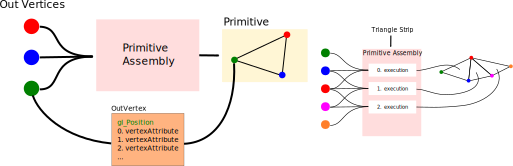
\includegraphics[width=12.5cm,keepaspectratio]{pics/pipeline/PrimitiveAssembly}
\end{frame}

\begin{frame}
\frametitle{Culling, clipping}
  \scriptsize
	\begin{itemize}
		\item Clipping, Culling, Perspective Divide and Viewport Transformation is performed between primitive assembly unit and rasterization.
    \item Culling discards back facing triangles.
    \item Clipping clips triangles that are not completely inside view-frustum.
    \item Perspective division shrinks objects that are further from the camera.
    \item Viewport Transformation transforms geometry to match screen resolution.
	\end{itemize}
	\begin{itemize}
    \item Mezi rasterizací a sestavením primitiv se provádí ořez, zahazování odvrácených trojúhelníků, perspektivní dělení a viewport transformace.
    \item Clipping ořezává primitiva, která jsou jen částečně v pohledovém jehlanu.
    \item Perspektivní dělení zmenšuje objekty, které jsou dál od kamery.
    \item Viewport transformace převádí objekty na rozměr obrazovky.
	\end{itemize}
	
\includegraphics[width=12.5cm,keepaspectratio]{pics/pipeline/OpenGL460PipelineClipping}
\end{frame}

\begin{frame}
\frametitle{Culling}
  \scriptsize
	\begin{itemize}
		\item Culling removes triangles that are backfacing or front facing the camera.
    \item The state of triangle orientation is decided by vertex winding.
    \item It is possible to discard backfacing or frontfacing triangles.
    \item Is is also possible to specify what is backfacing side (clock wise/counter clock wise vertices).
    \item Just for 2 manifold objects or scenes with restricted camera movement.
    \item Performance can be doubled with Culling.
	\end{itemize}
	\begin{itemize}
		\item Culling se stará o zahazování odvrácených trojúhelníků.
    \item Odvrácenost je rozhodnuta na základě pořadí vrcholů.
    \item Je možné nastavit, jestli je trojúhelník přivrácený nebo odvrácený, pokud jsou vrcholy po nebo proti směru hodinových ručiček.
    \item Výkon vykreslování může být zdvojnásoben díky Cullingu.
	\end{itemize}
	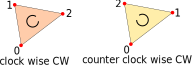
\includegraphics[width=8.5cm,keepaspectratio]{pics/pipeline/culling}
\end{frame}

\begin{frame}
\frametitle{Clipping, near-plane clipping}
  \scriptsize
	\begin{itemize}
		\item If a primitive is only partially inside view-frutum, it needs to be clipped.
    \item Only near-plane clipping is necessary.
    \item If the result is quadrangle, it can be replaced with two sub-triangles.
	\end{itemize}
	\begin{itemize}
		\item Pokud je primitivum jen částečně uvnitř pohledového jehlanu, je potřeba jej oříznout.
    \item Obvykle stačí oříznout pomocí blízké ořezové roviny (near-plane).
    \item Pokud vznikne čtyřúhelník, je možné jej nahradit dvěma trojúhelníky.
	\end{itemize}
	\begin{picture}(120,150)
		\put(0,0){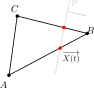
\includegraphics[width=4.5cm,keepaspectratio]{pics/pipeline/clip}}
	\end{picture}
	\begin{picture}(60,40)
		\put(25,0){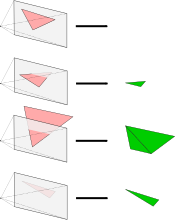
\includegraphics[width=4cm,keepaspectratio]{pics/pipeline/clip_variants}}
	\end{picture}
\end{frame}

\begin{frame}
\frametitle{Perspective Divide / Perspektivní dělení}
  \scriptsize
	\begin{itemize}
		\item Perspective Division unit converts hommogeneous coordinates to cartesian coordinates.
    \item It divides $x,y,z$ using $w$. The $w$ contains distance from camera.
    \item After division, $x,y,z \in [-1,+1]$ which is called normalized device coordinates (NDC).
    \item Division is expensive operation, specialized HW performs it fasters.
	\end{itemize}
	\begin{itemize}
		\item Blok perspektivního dělení převádí homogenní souřadnice na kartézské.
    \item Dělí se pomocí W, ve kterém je uložena hloubka. Tím se zmenšují objekty, které jsou dál od kamera.
    \item Po perspekvitním dělení všechny vrcholy leží v rozsahu $[-1,+1]$ - normalized device coordinates.
    \item Dělení je drahá operace, specializovaný HW ji provede rychleji.
	\end{itemize}
	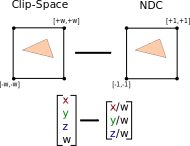
\includegraphics[width=6.5cm,keepaspectratio]{pics/pipeline/PerspectiveDivision}
\end{frame}

\begin{frame}
\frametitle{Viewport Transform / Viewport transformace}
  \scriptsize
	\begin{itemize}
		\item Viewport transformation converts NDC to screen resolution.
	\end{itemize}
	\begin{itemize}
		\item Blok viewport transformace transformuje normalizované souřadnice na rozlišení plátna.
	\end{itemize}
	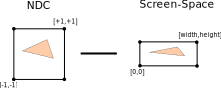
\includegraphics[width=8.5cm,keepaspectratio]{pics/pipeline/ViewportTransformation}
\end{frame}

\begin{frame}
\frametitle{Tessellation / Teselace}
  \scriptsize
	\begin{itemize}
		\item Tessellation is composed of 2 programable parts and hardware primitive generator.
    \item The goal of tessellation is to add geometric details.
	\end{itemize}
	\begin{itemize}
		\item Tesselace je složena zde 2 programovatelných processorů a hardwarového generátoru primitiv.
    \item Cíl teselace je přidání geometrických detailů.
	\end{itemize}
	
\includegraphics[width=12.5cm,keepaspectratio]{pics/pipeline/OpenGL460PipelineTessellationShaders}
\end{frame}

\begin{frame}
\frametitle{Geometry processor, transform feedback}
  \scriptsize
	\begin{itemize}
		\item Geometry processor inputs and outputs are primitives.
    \item The goal is to change, generate primitives.
    \item The stream of primitives can be sent to buffer.
	\end{itemize}
	\begin{itemize}
		\item Geometry processor transformuje primitiva.
    \item Transform feedback může primitiva přeposlat zpět do bufferu.
	\end{itemize}
	
\includegraphics[width=12.5cm,keepaspectratio]{pics/pipeline/OpenGL460PipelineGeometryShader}
\end{frame}

\begin{frame}
\frametitle{Rasterization / Rasterizace}
  \scriptsize
	\begin{itemize}
		\item Rasterization produces fragments.
    \item Fragment is date structure that is created in the location of sampling point.
    \item Sampling point is usualy in the center of pixel.
    \item The situation is more complicated with the use of multisampling.
    \item If a sampling point is located inside a triangle, a fragment is created for corresponding pixel.
	\end{itemize}
	\begin{itemize}
		\item Rasterizace produkuje fragmenty.
    \item Fragment je datová struktura, která vznikne na pozici vzorku (sampling point).
    \item Vzorkovací bod je obvykle uprostřed pixelu.
    \item Situace je komplikovanější při využití multi-samplingu.
    \item Pokud leží vzorkovací bod uvnitř trojúhelníku, vznikne fragment pro daný pixel.
	\end{itemize}
	\begin{figure}[h]
		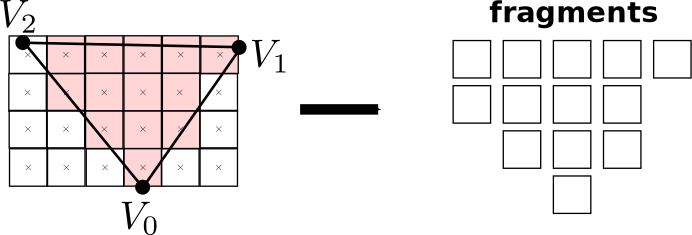
\includegraphics[width=10cm,keepaspectratio]{pics/pipeline/rasterization.pdf}
	\end{figure}
\end{frame}

\begin{frame}
\frametitle{Rasterization and Interpolation / Rasterizace a interpolace}
  \scriptsize
	\begin{itemize}
		\item Out Vertices are composed of n vertex attributes.
    \item Rasterization produces fragments -- data structure -- which is composed of fragment attributes with the same user specific fragment attributes.
    \item Barycentric interpolation is used to transform three vertex data structures to many fragment data structures.
	\end{itemize}
	\begin{itemize}
		\item Vertexy jsou před rasterizací popsány pomocí n-tice atributů
    \item Rasterizace produkuje fragmenty, pokud jejich střed leží uvnitř primitiva
    \item Po rasterizaci jsou tyto atributy vloženy do fragmetů pomocí interpolace
	\end{itemize}
	\begin{figure}[h]
		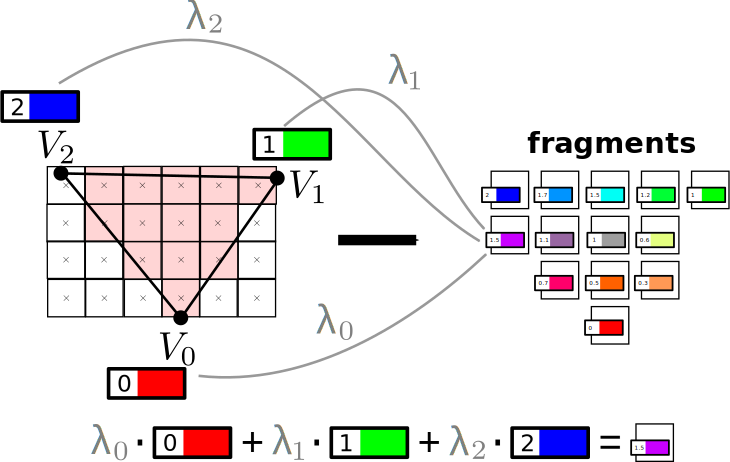
\includegraphics[width=10cm,keepaspectratio]{pics/pipeline/interpolation.pdf}
	\end{figure}
\end{frame}

\begin{frame}
\frametitle{Barycetric coordinates / Barycentrické koordináty}
	\begin{figure}[h]
		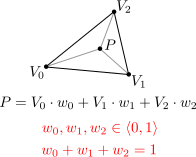
\includegraphics[width=8cm,keepaspectratio]{pics/pipeline/barycentrickekoordinaty.pdf}
	\end{figure}
\end{frame}

\begin{frame}
\frametitle{2D Barycentric coordinates / Barycentrické koordináty ve 2D}
  \scriptsize
	\begin{itemize}
		\item 2D barycentrics are computed as ratio between the area of the triangle and the areas of its sub-triangles. 
	\end{itemize}
	\begin{itemize}
		\item Barycentrické koordináty ve 2D jsou spočítaný jako poměr obsahů.
	\end{itemize}
	\begin{figure}[h]
		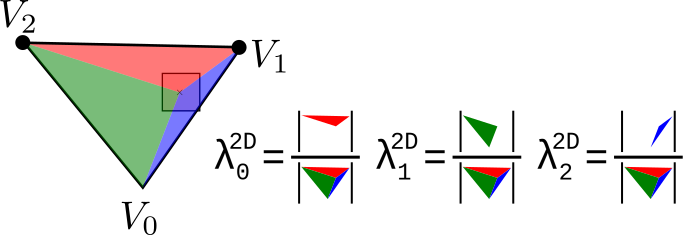
\includegraphics[width=8cm,keepaspectratio]{pics/pipeline/barycentric2D.pdf}
	\end{figure}
\end{frame}

\begin{frame}
\frametitle{Perspective distortion / Perspektivní zkreslení}
  \scriptsize
	\begin{itemize}
		\item Vertex attributes can be interpolated in the projection plane or in the 3D space.
    \item Interpolation in the 3D space is correct.
    \item In order to convert 2D interpolation to 3D interpolation, the perspective correction is required (OpenGL supports this natively / can be turned off)
	\end{itemize}
	\begin{itemize}
		\item Vertex atributy se mohou interpolovat v rovině průmětny nebo v prostoru scény
    \item Aby se mohlo interpolovat v prostoru scény, musí se provést perspektivní korekce
      (v OpenGL automaticky/lze vypnout)
	\end{itemize}
	\begin{figure}[h]
		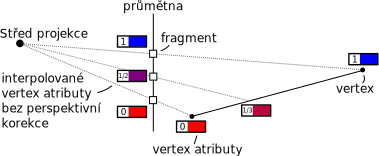
\includegraphics[width=10cm,keepaspectratio]{pics/pipeline/prespektivni_korekce.pdf}
	\end{figure}
\end{frame}

\begin{frame}
\frametitle{Fragment Processor}
  \scriptsize
	\begin{itemize}
		\item Fragment shader is executed inside fragment processor.
    \item Fragment Shader is user program.
    \item The goal of the shader is to transform input fragment to output fragments.
    \item Multiple Render Target - support for rendering into multiple 2D arrays (renderbuffers / textures).
	\end{itemize}
	\begin{itemize}
		\item Ve Fragment Processoru běží fragment shader.
    \item Fragment Shader je uživatelem specifikovaný program.
    \item Cílem je transformovat vstupní fragment na výstupní fragment.
    \item Multiple Render Target.
	\end{itemize}
	\begin{figure}[h]
		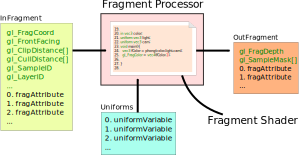
\includegraphics[width=8cm,keepaspectratio]{pics/pipeline/FragmentShader.pdf}
	\end{figure}
\end{frame}

\begin{frame}
\frametitle{Early fragment tests / Brzké testy a operace}
	\begin{figure}[h]
	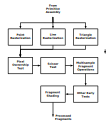
\includegraphics[width=7cm,keepaspectratio]{pics/pipeline/OpenGL460PipelineRaster}
	\end{figure}
\end{frame}

\begin{frame}
\frametitle{Late fragment tests and operations}
	\begin{figure}[h]
	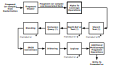
\includegraphics[width=12.5cm,keepaspectratio]{pics/pipeline/OpenGL460PipelineFragmentShader}
	\end{figure}
\end{frame}

\begin{frame}
\frametitle{PFO - depth test}
	\begin{figure}[h]
	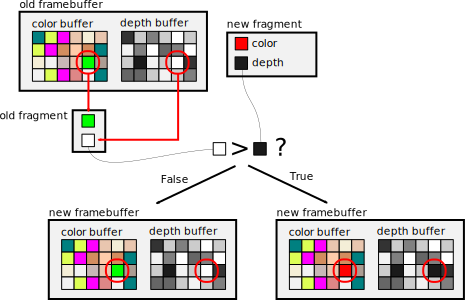
\includegraphics[width=10.5cm,keepaspectratio]{pics/pipeline/PFO}
	\end{figure}
\end{frame}


\begin{frame}
\frametitle{OpenGL 4.6 pipeline}
  \begin{figure}[h]
  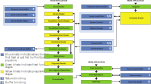
\includegraphics[width=10cm,keepaspectratio]{pics/pipeline/OpenGL460Pipeline}
  \end{figure}
\end{frame}



\bluepage{OpenGL}

\begin{frame}
\frametitle{OpenGL}
  \begin{itemize}
  \item OpenGL Open Graphics Language (Library) 
  \item OpenGL je API pro 3D grafiku 
  \item Vychází z IrisGL od SGI 
  \item Platformně nezávislé 
  \item Použitelné skoro z každého jazyka 
  \item Slouží pro převod scény popsané primitivy (body, čáry trojúhelníky)  na 2D rastr obrazovky.
  \item V novější verzi (4.3) i pro GPGPU
  \item Obsahuje vlastní jazyk GLSL pro programování GPU
  \end{itemize}
  \begin{figure}[h]
  
\includegraphics[width=5cm,keepaspectratio]{pics/opengl/logo}
  \end{figure}
\end{frame}

\begin{frame}
\frametitle{OpenGL - proč používat?}
  \begin{itemize}
    \item{OpenGL je multiplatformní - Linux, Window, Mac Os X, Android,...}
    \item{OpenGL lze použít téměř z každého jazyka - C, C++, Python, Java, Javascript, ...}
    \item{OpenGL je zpětně kompatibilní}
    \item{OpenGL je nízkoúrovňové}
    \item{OpenGL má jednoduché API}
    \item{OpenGL je rychlé}
    \item{OpenGL je otevřený industriální standard}
    \item{WebGL}
  \end{itemize}
\end{frame}


\begin{frame}
\frametitle{Verze OpenGL}
  \begin{itemize}

  \item{OpenGL}
  \begin{itemize}
  \item{1.x - fixní pipeline}
  \item{\textbf{2.x} - programovatelná pipeline}
  \item{3.x - geometry shader, \textbf{Deprecation}}
  \item{4.x - Hardwarová tesselace, dvojitá přesnost}
  \item{4.3 - Compute shadery}
  \item{4.5 - Direct State Access}
  \end{itemize}

  \item{OpenGL ES}
  \begin{itemize}
  \item{Vestavěné systémy, mobily, tablety}
  \item{1.x - fixní pipeline}
  \item{\textbf{2.x} - programovatelná pipeline}
  \item{3.x - Occlusion queries, 3D textury, transform feedback}
  \end{itemize}

  \item{WebGL}
  \begin{itemize}
  \item{OpenGL ve webovém prohlížeči}
  \item{\textbf{Velmi podobné OpenGL ES}}
  \end{itemize}

  \end{itemize}
\end{frame}

\begin{frame}
\frametitle{OpenGL}
  \begin{itemize}
    \item{OpenGL je architektura klient server}
    \item{Aplikace běží na CPU a využívá OpenGL pro přístup k GPU}
  \end{itemize}
  \begin{figure}[h]
    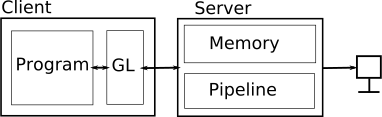
\includegraphics[width=10cm,keepaspectratio]{pics/opengl/clientserver}
  \end{figure}
\end{frame}

\begin{frame}
\frametitle{OpenGL}
	\begin{picture}(320,250)
		\put(-25,70){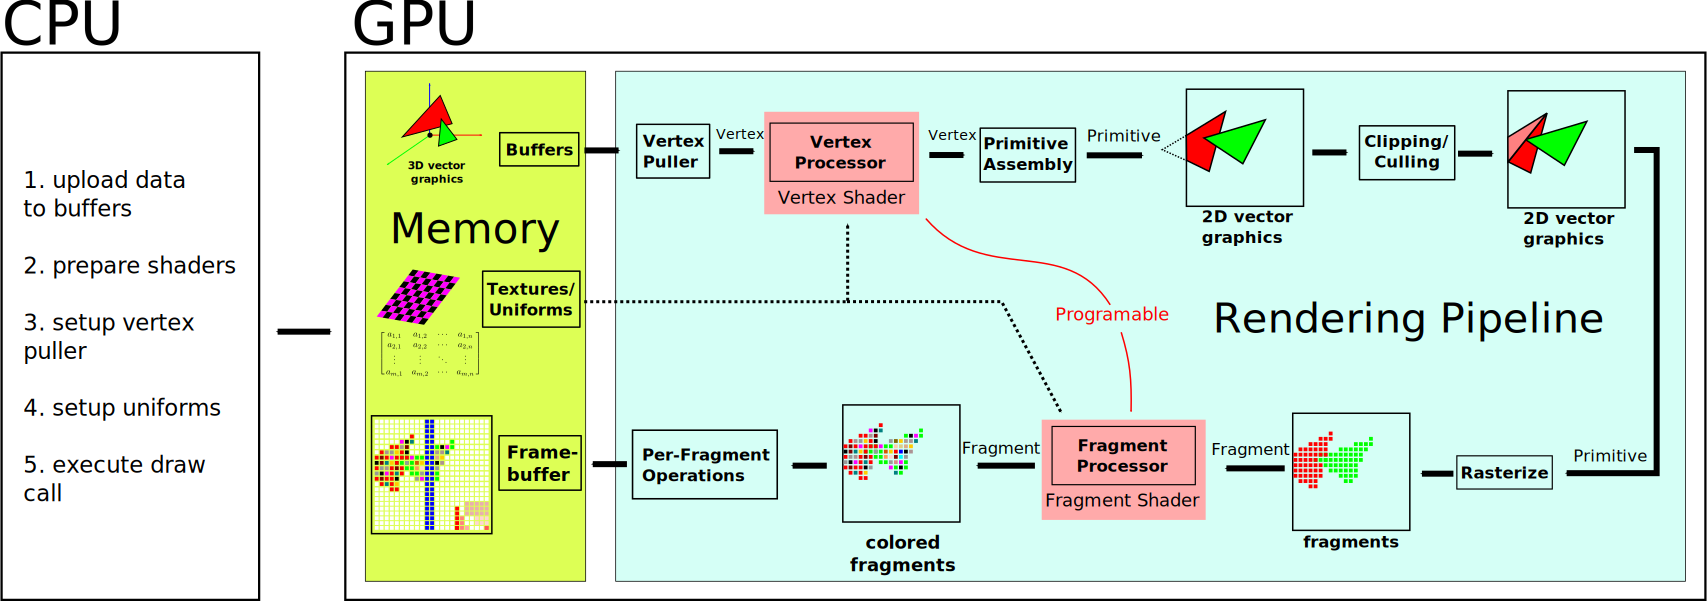
\includegraphics[width=12.5cm,keepaspectratio]{pics/opengl/RenderingPipeline}}
	\end{picture}
\end{frame}

\begin{frame}
\frametitle{OpenGL API}
  \begin{itemize}
    \item Jednoduché rozhraní
      \begin{itemize}
        \item Pouze C funkce
        \item Data jsou jen čísla a pole
        \item Žádné struct, class
      \end{itemize}
    \item Stavový stroj
      \begin{itemize}
        \item Většina příkazů nastavuje stav pipeline
        \item Stav se sám nemění
      \end{itemize}
    \item OpenGL (Rendering) Context
      \begin{itemize}
        \item Hlavní objekt OGL
        \item Mimo OpenGL (WGL/GLX)
        \item Zapouzdřuje data, stav, napojení na výstup
      \end{itemize}
  \end{itemize}
\end{frame}

\begin{frame}
\frametitle{Příkazy a typy}
  glName{\it NT}(...)
  \begin{itemize}
    \item N - počet parametrů
    \item T - typ parametrů
  \end{itemize}
    \begin{tabular}{|l|l|l|l|}
    \hline
    b & 8b integer & signed char & GLbyte \\ \hline
    s & 16b integer & short & GLshort \\ \hline
    i & 32b integer & long & GLint,GLsizei \\ \hline
    f & 32b float & float & GLfloat,GLclampf \\ \hline
    d & 64b float & double & GLdouble,GLclampd \\ \hline
    ub & 8b unsigned & unsigned char & GLubyte,GLboolean \\ \hline
    us & 16b unsigned & unsigned short & GLushort \\ \hline
    ui & 32b unsigned & unsigned long & GLuint,GLenum,GLbitfield \\ \hline
    *v & Ukazatel a * & & \\ \hline
    \end{tabular}
    GLvoid glUniform2f(GLuint,GLfloat,GLfloat);
    GLvoid glUniform2fv(GLuint,GLfloat*);
\end{frame}

\begin{frame}
\frametitle{Příkazy a typy}
  OpenGL příkazy lze rozdělit do několika skupin
  \begin{itemize}
    \item \textbf{Příkazy pro správu OpenGL objektů (10 hlavních OpenGL objektů)}
    \item \textbf{Exekuční příkazy (kreslící a výpočetní příkazy)}
    \item \textbf{Stavové příkazy (nastavují globální stav OpenGL, příkazy pro zjištění stavu)}
    \item Debugovací příkazy
    \item Operace s framebufferem
    \item Příkazy pro synchronizaci (glFinish)
    \item Utilitní příkazy
  \end{itemize}
\end{frame}


\begin{frame}
\frametitle{OpenGL Objekty}
  GLvoid glGen{\it Objects}(GLsizei n,GLuint * objects);\\
  GLvoid glDelete{\it Objects}(GLsizei n,const GLuint * objects);
  \begin{itemize}
    \item Jméno objektu - GLuint, všechny objekty jsou v API reprezentovány integerem
    \item 0 rezervována pro prázdný objekt
  \end{itemize}
  Objekty:
  \begin{itemize}
    \item \textbf{Program}
    \item \textbf{Shader}
    \item \textbf{Buffer}
    \item \textbf{Vertex Array Object}
    \item Texture
    \item Framebuffer
    \item Renderbuffer
    \item Sampler
    \item Asynchronous Query
    \item ProgramPipeline
  \end{itemize}
\end{frame}

\begin{frame}
\frametitle{Způsob využití OpenGL pro kreslení}
  \begin{itemize}
    \item Pro vykreslení grafiky pomocí OpenGL je potřeba inicializovat několik objektů
    \item Shader Program(y), Buffer(y), Vertex Array Object(y)
    \item Inicializace spočívá v kompilaci a likování programů
    \item Alokaci a kopírování dat na GPU
    \item Konfigurace stavů OpenGL a konfigurace čtení z GPU paměti
    \item Spuštění kreslení pomocí vykreslovacích příkazů
  \end{itemize}
\end{frame}



\bluepage{Shaders and Shader Programs}

\begin{frame}\frametitle{Two languages are needed / jsou potřeba dva jazyky}
\scriptsize
\begin{itemize}
  \item OpenGL standard describes API and OpenGL shading language -- GLSL.
  \item GLSL describes structure of programs running on GPU.
  \item Programmer needs to write the code in two languages -- one for CPU and one for GPU.
\end{itemize}

\begin{itemize}
  \item OpenGL standard popisuje i jazyk GLSL.
  \item Jazyk GLSL popisuje programy, které běží na GPU.
  \item Programátor 3D grafiky píše aplikaci vždy ve 2 jazycích.
\end{itemize}
  \begin{figure}[h]
    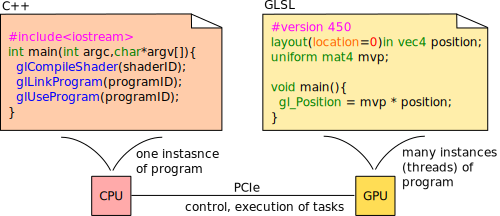
\includegraphics[width=10cm,keepaspectratio]{pics/program/cpp_and_glsl.pdf}
  \end{figure}
\end{frame}

\begin{frame}\frametitle{Shader programs, Shaders}
\scriptsize
\begin{itemize}
\item A shader program is program that runs on GPU.
\item Shader Program is composed of few stages called shaders.
\item There are six shader types: \textbf{vertex}, \textbf{fragment}, geometry, tesselation control, tesselation evaluation and compute shader.
\item Shader program does not have to contain all stages.
\item Stages can be shared among multiple programs.
\item Shaders can be precompiled or compiled in runtime.
\item Shader programs are linked.
\end{itemize}

\begin{itemize}
\item Program, který běží na GPU se v OpenGL označuje jako shader program.
\item Shader Program je složen z několika částí (stages), které se nazývají shader.
\item Existuje 6 typů shaderů: \textbf{vertex}, \textbf{fragment}, geometry, tesselation control, tesselation evaluation a compute shader.
\item Program nemusí obsahovat všechny typy shaderů.
\item Jednotlivé shadery lze sdílet mezi vícero programy.
\item Shadery se kompilují (za běhu aplikace).
\item Programy se linkují (za běhu aplikace), ale mohou být předpřipraveny v binárce.
\end{itemize}
\end{frame}

\begin{frame}\frametitle{Shader combinations / Kombinace shaderů v programu}
  Valid and commonly used shader combinations:\\
  Validní a často používané kombinace shaderů:
  \begin{figure}[h]
    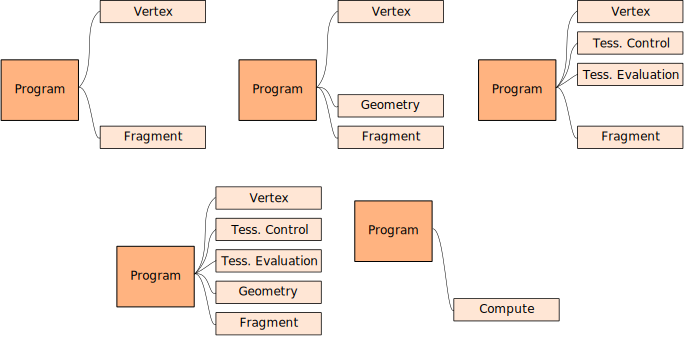
\includegraphics[width=10cm,keepaspectratio]{pics/program/shader_combination.pdf}
  \end{figure}
\end{frame}

\begin{frame}[fragile]\frametitle{Shader compilation / Kompilace shaderů}\scriptsize
\begin{minted}[bgcolor=bg]{packages/c_cpp.py:CppLexer -x}
GLuint createShader(GLuint type, std::string const& src) {
  //create handle
  GLuint id = glCreateShader(type);

  //set shader source
  char const* vsSrc[1] = {
    src.c_str()
  };
  glShaderSource(id, 1, vsSrc, nullptr); 

  //compile shader
  glCompileShader(id);

  //get compilation status
  int compileStatus;
  glGetShaderiv(id, GL_COMPILE_STATUS, &compileStatus);
  if (compileStatus != GL_TRUE) {
    //get message info length
    GLint msgLen;
    glGetShaderiv(id,GL_INFO_LOG_LENGTH,&msgLen);
    auto message = std::string(msgLen,' ');
    // get message
    glGetShaderInfoLog(id, msgLen, nullptr, message.data());
    std::cerr << message << std::endl;
  }
  return id;
}
\end{minted}
\end{frame}

\begin{frame}[fragile]\frametitle{Program linking}\scriptsize
\begin{minted}[bgcolor=bg]{packages/c_cpp.py:CppLexer -x}
GLuint createProgram(std::vector<GLuint>const& shaders) {
  //create handle
  GLuint prg = glCreateProgram();

  //attach shaders
  for(auto const&shader:shaders)
    glAttachShader(prg,shader);

  //link program
  glLinkProgram(prg);

  //get link status
  GLint linkStatus;
  glGetProgramiv(prg, GL_LINK_STATUS, &linkStatus);
  if(linkStatus != GL_TRUE){
    //get message info length
    GLint msgLen;
    glGetProgramiv(prg,GL_INFO_LOG_LENGTH,&msgLen);
    auto message = std::string(msgLen,' ');
    glGetProgramInfoLog(prg, msgLen, nullptr, message.data());
    std::cerr << message << std::endl;
  }
  return prg;
}
\end{minted}
\end{frame}

\begin{frame}[fragile]\frametitle{1 Triangle example / ukázka jednoho trojúhelníku}\scriptsize
\begin{minted}[bgcolor=bg]{packages/c_cpp.py:CppLexer -x}

int main(int32_t argc,char*argv[]){
  ...
  // vertex shader source
  auto vsSrc = R".(
  #version 460
  void main(){
    gl_Position=vec4(gl_VertexID&1,gl_VertexID>>1,0,1);
  }
  ).";

  // fragment shader source
  auto fsSrc = R".(
  #version 460
  out vec4 fColor;
  void main(){
    fColor = vec4(1);
  }
  ).";

  GLuint vs = compileShader(GL_VERTEX_SHADER  ,vsSrc);
  GLuint fs = compileShader(GL_FRAGMENT_SHADER,fsSrc);
  GLuint program = createProgram({vs,fs});
}
\end{minted}
\end{frame}



\begin{frame}\frametitle{GLSL}\scriptsize
\begin{itemize}
  \item GLSL - OpenGL Shading Language.
  \item It describes programs that are executed on GPU.
  \item C based.
  \item No recursion, classes, exceptions, std libs.
  \item Vector and matrix types, built-in variables and functions, synchronzation, variable qualifiers, swizzling.
  \item Every shader stage must have main function - entry point.
  \item Shader is execute in many instances -- threads in particular stage of pipeline
  \item Some parts of pipeline have special setttings.
\end{itemize}

\begin{itemize}
  \item GLSL - OpenGL Shading Language.
  \item Slouží pro popis programů, které běží na GPU.
  \item Je odvozený od C.
  \item Neobsahuje rekurzi, třídy, výjimky, std knihovny.
  \item Obsahuje vektorové a maticové typy, vestavěné funkce, vestavěné proměnné, synchronizační funkce, kvalifikátory, rozšířené adresování vektorů.
  \item Každý shader musí obsahovat main funkci.
  \item Každá main funkce je vykonávána v mnoha instancích v dané části pipeline.
  \item Některé části pipeline mají speciální nastavení.
\end{itemize}
\end{frame}

\begin{frame}[fragile]\frametitle{Types, swizzling / typy, swizzling}\scriptsize
\begin{minted}[bgcolor=bg]{packages/graphics.py:GLShaderLexer -x}
#version 450

void main(){
  //32 bit integer
  int a;
  //32 bit unsigned integer
  uint b;
  //32 bit float
  float c;
  //vector of 4 ints
  ivec4 d;
  //vector of 3 floats
  vec3 e = vec3(1,2,3);
  //matrix 3x3 of floats
  mat3 m;
  //zeroth element of e
  e[0] == e.x == e.r;
  //swizzling 
  vec2 f = e.xy; // (1,2)
  f = e.zz; // (3,3)
  //matrix vector multiplication
  e = m*e;
  //constructing ivec4 from vec3 and scalar
  d = ivec4(c,4);
  d = ivec4(c.xx,c.yy);
}
\end{minted}
\end{frame}

\begin{frame}[fragile]\frametitle{Built-in functions / vestavěné funkce}\tiny
\begin{minted}[bgcolor=bg]{packages/graphics.py:GLShaderLexer -x}
abs acos acosh asin asinh atan atanh ceil cos cosh degrees exp exp2 floor fract inversesqrt
log log2 max min mod modf pow radians round roundEven sign sin sinh sqrt tan tanh trunc
clamp cross distance dot floatBitsToInt floatBitsToUint fma frexp intBitsToFloat isinf
isnan ldexp length mix normalize smoothstep step

packDouble2x32 packSnorm4x8 packUnorm2x16 packSnorm2x16
packUnorm4x8 uintBitsToFloat unpackDouble2x32 unpackSnorm4x8 unpackUnorm2x16 
unpackSnorm2x16 unpackUnorm4x8 packHalf2x16 unpackHalf2x16

all any bitCount bitfieldExtract bitfieldInsert bitfieldReverse determinant equal
faceforward findLSB findMSB greaterThan greaterThanEqual imulExtended inverse lessThan
lessThanEqual matrixCompMult not notEqual outerProduct reflect refract transpose uaddCarry
umulExtended usubBorrow 

textureSize textureQueryLod texture textureProj textureLod 
textureOffset texelFetch texelFetchOffset textureProjOffset textureLodOffset textureProjLod 
textureProjLodOffset textureGrad textureGradOffset textureProjGrad textureProjGradOffset 
textureGather textureGatherOffset textureGatherOffsets textureQueryLevels

dFdx dFdy fwidth
interpolateAtCentroid interpolateAtOffset interpolateAtSample

noise1 noise2 noise3 noise4

EmitStreamVertex EndStreamPrimitive EmitVertex EndPrimitive

barrier memoryBarrier 
memoryBarrierAtomicCounter memoryBarrierBuffer memoryBarrierImage memoryBarrierShared 
groupMemoryBarrier
imageSize

atomicAdd atomicMin atomicMax atomicAnd atomicOr atomicXor atomicExchange atomicCompSwap

imageSize imageLoad imageStore imageAtomicAdd imageAtomicMin imageAtomicMax
imageAtomicAnd imageAtomicOr imageAtomicXor imageAtomicExchange imageAtomicCompSwap
\end{minted}
\end{frame}

\begin{frame}[fragile]\frametitle{Variable qualifiers / kvalifikátory proměnných}\tiny
\begin{minted}[bgcolor=bg]{packages/graphics.py:GLShaderLexer -x}
#version 450

//data comes from previous stage (or buffer in case of vertex shaders)
//read only
in vec4 a;

//data is sent to next stage
out vec4 b;

//a,b variables are different for every shader invocation

//data is constant, all threads see the same value, can be set from CPU
uniform mat4 m;

//opaque type d (texture), can be accessed through specialized functions
//read only
uniform sampler2D d;

//local variable stored in registers 
//every thread has its own
vec4 e = vec4(0,1,2,3);

void main(){
  b = e + m * texture(d,a.xy);
}
\end{minted}
\end{frame}

\begin{frame}[fragile]\frametitle{Vertex Shader built-ins / vestavěné proměnné VS}
Vertex Shader contains some important built-in variables.\\
Vertex Shader obsahuje několik důležitých vestavěných proměnných.
{\scriptsize
\begin{minted}[bgcolor=bg]{packages/graphics.py:GLShaderLexer -x}
#version 450

void main(){
  //output variable - contain position of vertex in clip-space
  vec4 gl_Position;

  //vertex/index number
  in int gl_VertexID;
  //instance number
  in int gl_InstanceID;
  //draw call number
  in int gl_DrawID;
  //point size
  out float gl_PointSize;
  //distance to custom clip plane
  out float gl_ClipDistance[];
  out float gl_CullDistance[];
}

\end{minted}
}
\end{frame}

\begin{frame}[fragile]
\frametitle{Fragment built-ins / vestavěné progměnné FS}
Output of fragment shader is specified manually.\\
Výstup fragment shaderu si specifikuje programátor pomocí vlastní výstupní proměnné.
{\scriptsize
\begin{minted}[bgcolor=bg]{packages/graphics.py:GLShaderLexer -x}
#version 450

//output, 0. color buffer of framebuffer
layout(location=0)out vec4 fColor;

void main(){
  //fragment coordinates (x,y in screen resolution)
  in vec4 gl_FragCoord;

  //Was this fragment rasterized from front facing side of a triangle?
  in bool gl_FrontFacing;

  //this variable can modify depth of fragment.
  //writes disable early depth test (can be re-enabled)
  out float gl_FragDepth;

  in float gl_ClipDistance[];
  in float gl_CullDistance[];
  in int gl_PrimitiveID;
}

\end{minted}
}
\end{frame}


\bluepage{Příprava bufferů}

\begin{frame}\frametitle{Buffers}
\scriptsize
\begin{itemize}
\item An buffer is memory block allocated in device memory of GPU.
\item It can contain any data.
\item The most common usecase is for storing vertices and indices.
\item A buffer can be part of Vertex Array (as vertex buffer or element buffer).
\item For general purposes, it can be bound to \textcolor{red}{GL\_SHADER\_STORAGE\_BUFFER}.
\item A buffer can be used for transform feedback.
\item There are also buffer textures.
\end{itemize}

\begin{itemize}
\item Buffer je objekt zastřešující lineární paměť na GPU.
\item Může obsahovat jakákoliv data.
\item Nejčastěji se používá pro uložení vrcholů geometrie (a jejich vlastností) a indexů na vrcholy.
\item Pro obecné použití může být připojen k \textcolor{red}{GL\_SHADER\_STORAGE\_BUFFER}.
\item Lze jej použít pro transform feedback a pro buffer textury.
\end{itemize}
\end{frame}

\begin{frame}
\frametitle{OpenGL 4.6 pipeline}
  \begin{figure}[h]
  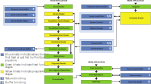
\includegraphics[width=10cm,keepaspectratio]{pics/pipeline/OpenGL460Pipeline}
  \end{figure}
\end{frame}

\definecolor{bg}{rgb}{0.95,0.95,0.95}

\begin{frame}[fragile]
\frametitle{Buffer creation, allocation, data upload}
Buffer creation / Vytvoření bufferu:
\scriptsize
\begin{minted}[bgcolor=bg]{packages/c_cpp.py:CppLexer -x}
float data[]={1,2};//CPU data
GLuint vbo;//buffer handle
glCreateBuffers(1,&vbo);
//allocate buffer and upload data
glNamedBufferData(vbo,sizeof(data),data,GL_DYNAMIC_DRAW);
\end{minted}
Buffer modification / Změna dat v bufferu.
\scriptsize
\begin{minted}[bgcolor=bg]{packages/c_cpp.py:CppLexer -x}
float*ptr;//pointer to data
ptr=(float*)glMapNamedBuffer(vbo,GL_READ_WRITE);//maps the buffer
ptr[0]=0.5;//sets the value
glUnmapNamedBuffer(vbo);//unmap buffer, commits changes
\end{minted}
Different way / Nebo pomoci {\color{blue} glNamedBufferSubData}.
    {\scriptsize
\begin{minted}[bgcolor=bg]{packages/c_cpp.py:CppLexer -x}
glNamedBufferSubData(vbo,
  sizeof(float),//offset
  sizeof(float),//size
  data);//data
    \end{minted}
    }
\end{frame}



\bluepage{Konfigurace Vertex Pulleru/Vertex Array Object}

\begin{frame}
\frametitle{Vertex Array Object}
  \begin{itemize}
  \item Vertex Array Object (VAO) obsahuje konfiguraci Vertex Puller jednoty.
  \item Vertex Puller čte data z bufferů a plní je do vstupních proměnných v prvním shaderu (vertex shader)
  \item VAO obsahuje nastavení propojení Shader Programu a Bufferů
  \item V novějších verzích OpenGL je povinný
  \item Obsahuje sadu nastavení pro každý Vertex Attribut a nastavení pro indexový buffer
  \item Jeden Vertex Attribut je napojen na jednu vstupní proměnnou ve Vertex Shaderu
  \item Mezi nastavení Vertex Attributu patří: číslo bufferu, velikost a typ datové položky, prokládání (stride), offset
  \end{itemize}
\end{frame}

\begin{frame}
\frametitle{Příklad - ilustrace 0. invokace vertex shaderu}
  \begin{figure}[h]
  \includegraphics[width=10cm,keepaspectratio]{pics/vao/puller0.pdf}
  \end{figure}
\end{frame}

\begin{frame}
\frametitle{Příklad - ilustrace 1. invokace vertex shaderu}
  \begin{figure}[h]
  \includegraphics[width=10cm,keepaspectratio]{pics/vao/puller1.pdf}
  \end{figure}
\end{frame}

\begin{frame}[fragile]
\frametitle{VAO - příklad}
{\scriptsize
\begin{minted}[bgcolor=bg]{packages/c_cpp.py:CppLexer -x}
GLuint vao;
glCreateVertexArrays(1,&vao);//vygenerovani jmena VAO
//nyni nastavime buffery a atributy

glVertexArrayAttribBinding(vao,0,0);
glEnableVertexArrayAttrib(vao,0);
glVertexArrayAttribFormat(vao,
  0,//cislo vertex attributu
  2,//pocet polozek pro cteni (vec2)
  GL_FLOAT,//typ polozek
  GL_FALSE,//normalizace
  0);//relativni offset
glVertexArrayVertexBuffer(vao,0,
  vbo,
  sizeof(float)*5,//stride
  (GLvoid*)(sizeof(float)*0));//offset

glVertexArrayAttribBinding(vao,1,1);
glEnableVertexArrayAttrib(vao,1);
glVertexArrayAttribFormat(vao,1,3,GL_FLOAT,GL_FALSE,0);
glVertexArrayVertexBuffer(vao,1,vbo,sizeof(float)*5,
  (GLvoid*)(sizeof(float)*2));

glVertexArrayAttribBinding(vao,2,2);
glEnableVertexArrayAttrib(2);
glVertexArrayAttribFormat(2,4,GL_FLOAT,GL_FALSE,0);
glVertexArrayVertexBuffer(vao,2,vbo,sizeof(float)*8,
  (GLvoid*)(sizeof(float)*10));
\end{minted}
}
\end{frame}

\begin{frame}[fragile]
\frametitle{VAO}
  \begin{figure}[h]
  \includegraphics[width=11cm,keepaspectratio]{pics/vao/vao.pdf}
  \end{figure}
\end{frame}


\bluepage{Kreslení a uniformní proměnné}

\begin{frame}[fragile]
\frametitle{Uniformní proměnné}
  \begin{itemize}
  \item Uniformní proměnné jsou uloženy v konstantní paměti
  \item Narozdíl od vertex atributů se v průběhu kreslení nemění
  \item Každá invokace shaderu adresuje stejnou hodnotu
  \item Uniformní proměnné lze využít ve všech shader stage
  \item Uniformní proměnné jsou vhodné například pro uložení matic, barvy, světla
  \item Stejně jako objekty v OpenGL zastupuje integerová hodnota, tak i každá uniformní proměnná má svoje integerové jméno
  \item Toto jméno lze získat z Shader Programu pomocí specializovaných funkcí
  \end{itemize}
\end{frame}

\begin{frame}[fragile]
\frametitle{Způsob využívání uniformních proměnných}
  \begin{enumerate}
  \item Vytvoření Shader Programu
  \item Získání integerového jména pomocí jména proměnné v shaderu
  \item Aktivování Shader Programu
  \item Nahrání dat pomocí vhodné OpenGL funkce
  \end{enumerate}
{\scriptsize
\begin{minted}[bgcolor=bg]{packages/c_cpp.py:CppLexer -x}
GLuint program = 0;
GLint  colorUniform = -1;
void init(){
  //sestaveni programu
  program = createProgram(
      compileShader(GL_VERTEX_SHADER  ,loadFile("flag.vp")),
      compileShader(GL_FRAGMENT_SHADER,loadFile("flag.fp")));
  //ziskani integeroveho jmena z promenne "color" v shaderu
  colorUniform = glGetUniformLocation(program,"color");
}
\end{minted}
}
{\scriptsize
\begin{minted}[bgcolor=bg]{packages/graphics.py:GLShaderLexer -x}
#verion 450

layout(location=0)out vec4 fColor;
uniform vec3 color;//uniformni promenna
void main(){
  fColor = vec4(color,1);
}
\end{minted}
}
\end{frame}


\begin{frame}[fragile]
\frametitle{Vykreslení dat}
  \begin{enumerate}
  \item Aktivování programu
  \item Nastavení uniformních proměnných
  \item Aktivování Vertex Array Objectu
  \item Zavolání vykreslovacího příkazu
  \end{enumerate}
{\scriptsize
\begin{minted}[bgcolor=bg]{packages/c_cpp.py:CppLexer -x}
void draw(){
  //vymazani barevneho framebuffer
  glClear(GL_COLOR_BUFFER_BIT);

  //aktivovani program
  glUseProgram(program);

  //nastaveni uniformni promenne
  glProgramUniform3fv(program,colorUniform,1,0,0);

  //aktivovani vao
  glBindVertexArray(vao);

  glDrawArrays(//vykresleni
    GL_TRIANGLES,//typ primitiva
    0,//prvni Vertex
    3);//pocet Vertexu pro vykresleni 3 -> 1 trojuhelnik

  //deaktivovani vao
  glBindVertexArray(0);
\end{minted}
}
\end{frame}


\bluepage{Per fragment operace}

\begin{frame}[fragile]
\frametitle{Per fragment operace}
  \begin{itemize}
  \item Po fragment shaderu jsou na fragmenty aplikovány Per fragment operace
  \item Nejzákladnější operací je řešení viditelnosti pomocí depth testu
  \item Viditelnost se v OpenGL řeší pomocí Depth Buffer (paměť hloubky)
  \item Další testy jsou Stencil test a Scissor test
  \item Mezi jiné operace patří Blending, který se využívá pro průhledné objekty
  \end{itemize}
\end{frame}


\begin{frame}[fragile]
\frametitle{Depth Test a Depth Buffer}
  \begin{itemize}
  \item Depth test řeší viditelnost pomocí Depth Bufferu a to na úrovni fragmentů
  \item Různé způsoby nastavení
  \item Přesnost depth bufferu není nekonečná (většinou 24 bitů)
  \item Častý problem depth bufferu je jev známý jako depth Fight
  \item Brzký depth test - depth test může předběhnout vykonávání fragment shaderu
  \item Brzký depth test se provádí tehdy, pokud se ve fragment shaderu nemodifikuje hloubka fragmetu
  \item Brzký depth test může značně urychlit kreslení
  \end{itemize}
  {\scriptsize
\begin{minted}[bgcolor=bg]{packages/c_cpp.py:CppLexer -x}
glEnable(GL_DEPTH_TEST);//zapneme depth test - nastavi se stav pipeline
glDepthFunc(GL_LEQUAL);//fragment s mensi nebo stejnou hloubkou projde
glDepthMask(GL_TRUE);//maskovani zapisu do depth bufferu
  \end{minted}
  }
\end{frame}

\begin{frame}[fragile]
\frametitle{Bleding - průhledné objekty}
  \begin{itemize}
  \item Blending umožňuje kombinovat novou barvu s již zapsanou barvou ve framebufferu
  \item Blending je řízen pomocí blendovací operace, source a destination faktorů
  \item Blendovací operace jsou sčítání, odčítání, min, max, ...
  \item Source faktor se aplikuje na barvu fragmentu
  \item Destination faktor se aplikuje na barvu již uloženou ve framebufferu
  \item Nutnost kreslit ve správném pořadí
  \end{itemize}
  \begin{figure}[h]
  \includegraphics[width=3cm,keepaspectratio]{pics/pfo/blending.jpg}
  \end{figure}
  {\scriptsize
\begin{minted}[bgcolor=bg]{packages/c_cpp.py:CppLexer -x}
glEnable(GL_BLEND);//zapneme blending
glBlendEquation(GL_FUNC_ADD);//barvy se budou scitat
glBlendFunc(GL_SRC_ALPHA,GL_ONE_MINUS_SRC_ALPHA);//nastavime zpusob michani
  \end{minted}
  }
\end{frame}


\bluepage{OpenGL context, libraries / kontext, knihovny}

\begin{frame}\frametitle{Libraries / Knihovny}\scriptsize
  \textbf{SDL2} - Simple Directmedia Layer
  \begin{itemize}
    \item IO, windows, sounds, threads, ...
    \item IO, okna, zvuky, vlákna, ...
  \end{itemize}
  \textbf{GLM} - GL mathematics
  \begin{itemize}
    \item Vector algebra, useful matematics
    \item Práce s vektory a maticemi
  \end{itemize}
  \textbf{GLEW} - OpenGL Extension Wrangler
  \begin{itemize}
    \item OpenGL extensions
    \item OpenGL rozšíření
  \end{itemize}
  GLEE - GL Easy Extension library\\
  GLFW - (IO, windows, ...)\\
  GEGL - FIT OpenGL C++ library\\
  STBi - image loading\\
  Imgui - OpenGL gui\\
  tiny gltf - gltf model loader
\end{frame}

\begin{frame}\frametitle{Extensions / rozšíření}\scriptsize
  \begin{itemize}
    \item{glext.h}
    \item{void*wglGetProcAddress(const char*name);}
    \item{void*glXGetProcAddress(const char*name);}
    \item{PFNGL{\it NECO}PROC glNeco=(PFN...)wglGetProcAddress("glSomething");}
    \item{glGetString(GL\_EXTENSIONS);}
    \item{GL\_XYZ\_name}
    \item{GL\_ARB\_multisample}
    \item{GL\_EXT\_blend\_func\_separate}
    \item{IBM,NV,ATI,SGIS,...}
    \item{GLEE/GLEW/GEGL/...}
  \end{itemize}
\end{frame}

\begin{frame}[fragile]\frametitle{OpenGL kontext}\scriptsize
  \begin{itemize}
    \item OpenGL context encapsulates all OpenGL settings.
    \item It stores all OpenGL objects (buffers, programs, textures, ...).
    \item After the deletion of OpenGL context, GPU data are no longer available.
    \item OpenGL context is not described in OpenGL specification, it is possible to create it using extern libraries.
    \item Context version, context flags, debug context, profiles.
  \end{itemize}
  \begin{itemize}
    \item OpenGL kontext zapouzdřuje věškeré nastavení OpenGL.
    \item Zastřešuje všechny objekty (buffer, programy, textury, ...).
    \item Po jeho uvolnění, nejsou již data na GPU přístupná.
    \item OpenGL kontext není popsán v OpenGL specifikaci a lze jej vytvořit z externích knihoven.
    \item Kontext má svoji verzi (vertex OpenGL), možnost aktivovat debugging, a různe profily.
  \end{itemize}
\end{frame}

\begin{frame}[fragile]\frametitle{SDL2 context / Vytvoření kontextu - SDL2}\scriptsize
\begin{minted}[bgcolor=bg]{packages/c_cpp.py:CppLexer -x}
SDL_Init(SDL_INIT_VIDEO);//init. video

//create window
SDL_Window*window = SDL_CreateWindow("sdl2",0,0,1024,768,
  SDL_WINDOW_OPENGL|SDL_WINDOW_SHOWN);

//setup context parameters
unsigned version = 450;//context version
unsigned profile = SDL_GL_CONTEXT_PROFILE_CORE;//context profile
unsigned flags   = SDL_GL_CONTEXT_DEBUG_FLAG;//context flags
SDL_GL_SetAttribute(SDL_GL_CONTEXT_MAJOR_VERSION, version/100    );
SDL_GL_SetAttribute(SDL_GL_CONTEXT_MINOR_VERSION,(version%100)/10);
SDL_GL_SetAttribute(SDL_GL_CONTEXT_PROFILE_MASK ,profile         );
SDL_GL_SetAttribute(SDL_GL_CONTEXT_FLAGS        ,flags           );

SDL_GLContext context = SDL_GL_CreateContext(window);//create context

glewExperimental=GL_TRUE;
glewInit();//initialisation of gl* functions
\end{minted}
\end{frame}



%
%\begin{frame}
  \frametitle{References}
  \begin{itemize}
    \item \url{http://www.opengl.org/sdk/docs/}
    \item \url{http://www.opengl.org/documentation/glsl/}
    \item \url{http://www.opengl.org/registry/}
    \item \url{http://www.khronos.org/opencl/}
    \item \url{https://wiki.libsdl.org/FrontPage}
    \item \url{http://developer.amd.com/wordpress/media/2013/07/AMD_Accelerated_Parallel_Processing_OpenCL_Programming_Guide-rev-2.7.pdf}
    \item \url{http://amd-dev.wpengine.netdna-cdn.com/wordpress/media/2012/10/Asynchronous-Shaders-White-Paper-FINAL.pdf}
  \end{itemize}
\end{frame}


%
%\bluepage{Thank you for your attention! \vspace{10 mm} Questions?}

\end{document}
